\chapter{Literature review}
\section{Bluetooth Low Energy}
First of all, before discussing what beacons are in depth, it is useful to point out and describe the protocol they use to transmit their data.\\
They use Bluetooth Low Energy, which is a branch of the Bluetooth protocol and as a name implies, it uses a lot less power. Bluetooth Low Energy uses less energy by keeping things simple. In fact, the beacons used in this project are supported by this particular protocol and therefore have a lifespan of years, which makes them extremely convenient compared to other sensors, because the battery can last a very long time and there is not a need for constant maintenance.\\
BLE reduce power consumption by only sending data as needed instead of maintaining a constant connection.
This means it is great for periodic updates like getting readings from a sensor but it is not so great for streaming audio or video. For now that is a job best left to classic Bluetooth or even better Wi-Fi.\\
The biggest reason why BLE is so great for DIY is the fact that companies like Apple and Google have made it so easy for developers to use, that someone writing an app for iOS or Android can easily add in BLE support without needing any special certification or contending with any legal hurdles.\\ 
Now a little bit about the architecture of the BLE stack.\\
The Bluetooth LE operates on what is known the general attribute (GATT Peripheral), as shown in Figure~\ref{fig:GattPeripheral}. It is a giant table of key value data where the keys are unique IDs and the values are any number of different things and they collect themselves together in logical groupings. Therefore a single device would be considered to implement a single profile.\\
Underneath that, there are a collection of one or more services. These services can be defined by a fully unique ID or UUID (128-bit) or by a 16-bit AssignedNumber. 
These services are generally logical groupings of functionality, so there could be a proximity service or a thermometer service, or a time service and underneath that service would be one or more characteristics that are the individual values that make up that logical functionality. These values can be of two types: Read or Write, or both at once. For example, the thermometer service will have a read-only characteristic which provides the temperature reading and will have a Write-only value which can be configured by the user to define the Unit the temperature is reported.\\
This GATT Peripheral configuration is also used by these tiny devices, called beacons, which they will be covered in more details in the next section.

	\begin{figure}[h!]
		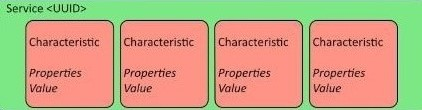
\includegraphics[width=1.0\textwidth]{GATT}
		\caption{GATT Peripheral explained in words previously. Here represented graphically}
		\label{fig:GattPeripheral}
	\end{figure}


\section{Beacons}
They are tiny devices which usually fit in the palm of a hand. They send different packages, using the BLE technology described previously, stating what they are, their signal strength and other characteristics. They are widely used for the following reasons.\\
\subsection{Platform Independent}
They are platform independent. Therefore, they are not bound by any companies or protocols.\\ 
Apple did, however, originally came out with the Ibeacon protocol, which led to some confusion whether Apple owned this technology or not and what the difference between beacons and Ibeacons were.\\
A beacon is the physical device with the antenna and the Bluetooth Low Energy stock which sends out packets. The Ibeacon is the layout of that packet. It is possible to have different layouts from different manufactures.
The Ibeacon is proprietary to Apple, but this does not mean they cannot be detected and used by android devices or other common operating systems.\\
\subsection{Not Internet Connected}
These beacons are not internet connected by default, they are not connected to WiFi and they are completely unaware of themselves and other devices around them.\\
They just sit there where they are mount and send out the information they are programmed to transmit for other devices to know they are in their proximity.\\
\subsection{Do Not Steal Data}
A beacon only sends out data. It is not capable of seeing other devices and cannot connect to them. Therefore, the user’s data and privacy are protected.\\
Furthermore, the user can receive those packets sent out by beacons, only after having opted-in, downloaded the appropriate app and set apposite permissions on their mobile phone.\\
Privacy is therefore not an issue and the user must not be concerned with it.\\
\subsection{They Can Detect Distance}
Beacons are okay at detecting distance. By measuring the received signal strength, which must be in the line of sight, it is possible to determine the user’s distance from that particular beacon with an approximation of +/- 1 metre, depending on the quality of the beacon and on the interferences present in the area.\\
Multiple beacons placed in a small environment, within close range between each other, will determine the exact location of the user. A similar process to the triangulation phase used by the GPS signals.\\
Depending on the beacon choice, the user can get a range from 2metres up to 70metres. This will affect the battery life. \\
However, the antenna power (TxPower) of each beacon can be adjusted to suit the individual use case and extend the battery life.\\
One disadvantage of using beacons for calculating distance however, is that it only works in foreground, especially in IOS. This means that it only works when the screen is on, it does not work when the screen is in stand-by. For the user this only means that if they need to obtain accurate location consistently, they must keep the phone’s screen on all the time.\\
\subsection{Come In Different Sizes}
These beacons come in different shapes and sizes. The choice of a particular beacon is up to each individual use case, on whether the sensor has to be placed outdoors, therefore it must be waterproof or whether the battery life is important, so the beacon must send packets at a low frequency, or whether it must be able to reach a wide range or if a short reach is enough.\\
Different manufactures provide with different beacons and their own product specifications.

	\begin{figure}[h]
		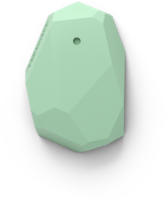
\includegraphics[scale = 1]{beacon}
		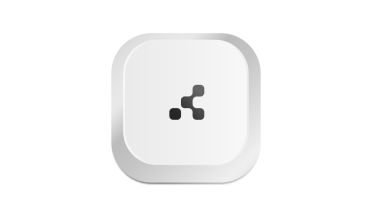
\includegraphics[scale = 1]{beacon1}
		\caption{These are pictures of different beacons. From left to right: Estimote beacon, Kontakt beacon}
		\label{fig:beacon}
	\end{figure}

\clearpage
\section{Beacon's protocols}
These beacons are simply physical devices; what makes them useful to users is the protocol they use to send data. There are different protocols available, but the 3 most used are: Ibeacon, Eddystone, AltBeacon.
\subsection{AltBeacon}
Altbeacon is an open source protocol designed and launched by Radius Network in July 2014. It was created to overcome the issue of protocols favouring one vendor over the other.\\
The advantages of this particular method over others available lies on its compatibility with different mobile platforms, its flexibility and its customizable source code.\\
The Altbeacon advertisement format makes use of the Manufacturer Specific Advertising Data structure as defined in the Bluetooth Specification Version 4.0. It is made up of a 1-byte length field, 1-byte type field and two-byte company identifier, followed by 24 additional bytes containing the beacon advertisement data, as shown in Figure~\ref{fig:altbeacon}.

	\begin{figure}[h]
		\centering
		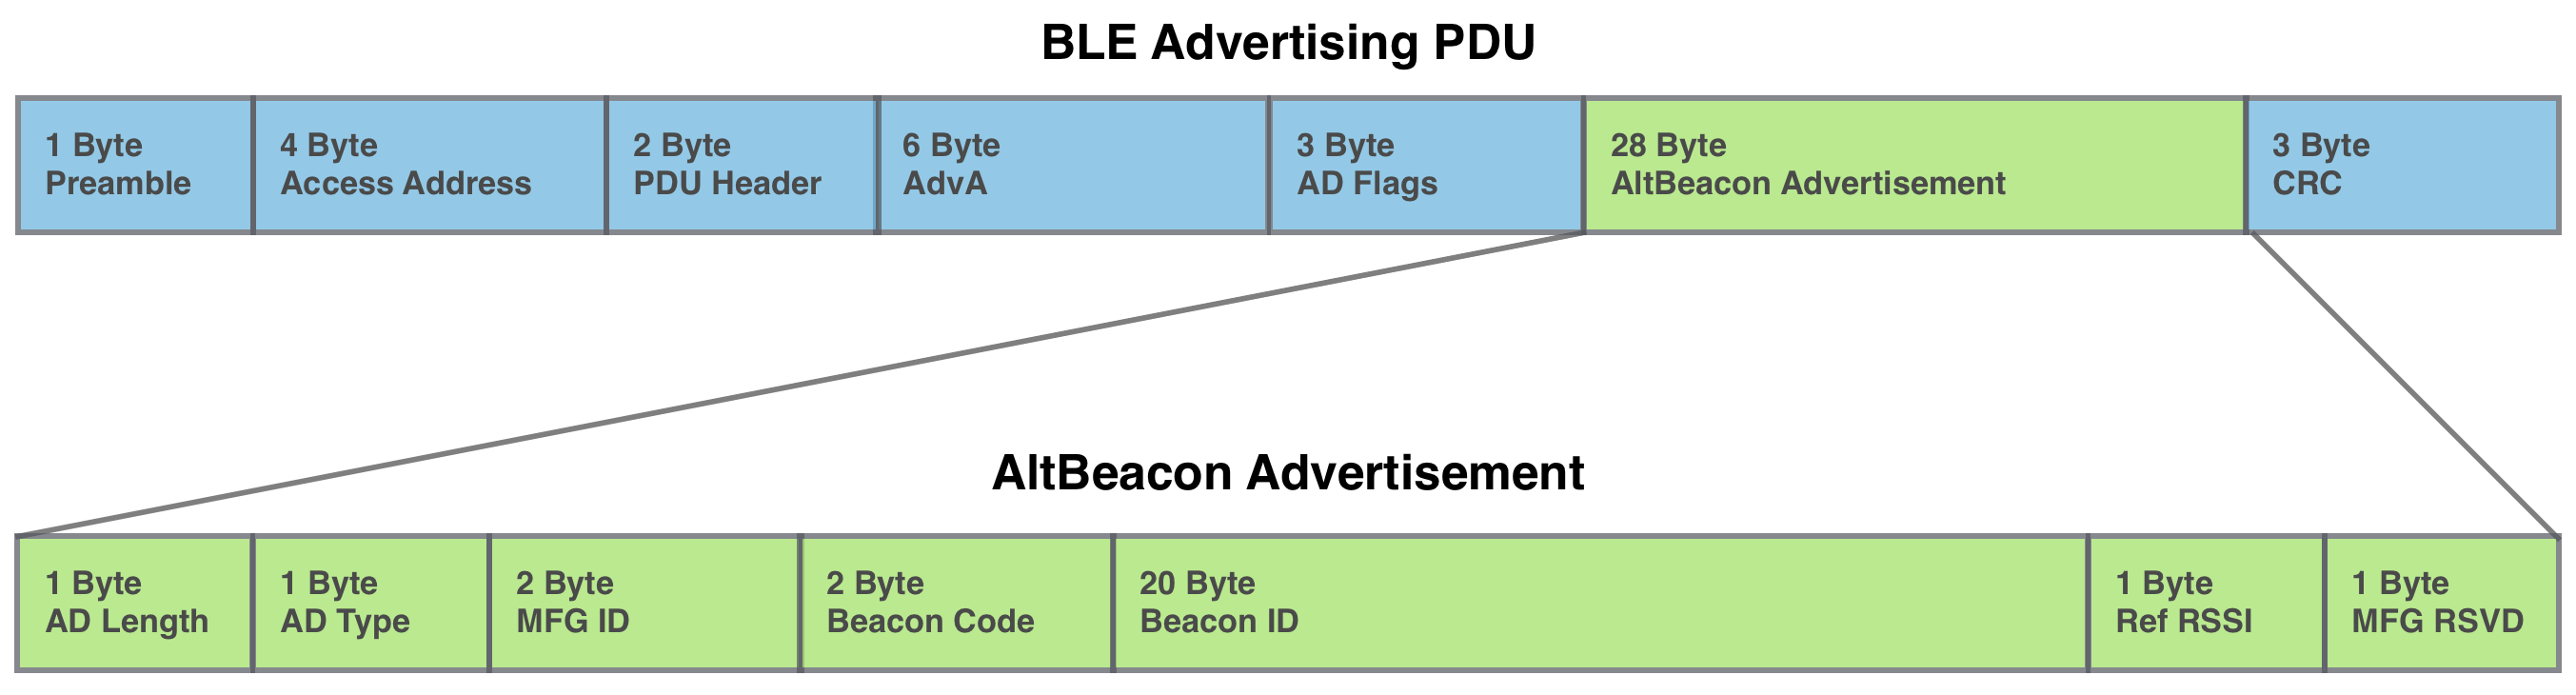
\includegraphics[scale = 0.345]{altbeacon}
		\caption{This diagram shows what the AltBeacon protocol is made up of.}
		\label{fig:altbeacon}
	\end{figure}

\subsection{Eddystone}
Eddystone is a protocol announced by Google in July 2015, after it was renamed from its former name UriBeacon.\\
As opposed to the Altbeacon frame, Eddystone can send three different packet types: Eddystone-UID (identifier), Eddystone-URL and Eddystone-TLM (telemetry). The former is similar to the UUID described in the previous sections: a 16 digit string of characters, which can identify the individual beacon and, while in range, can activate the Mobile App. The ladder (TLM) refers to the administrative data from the beacon itself communicated through telemetry, such as battery life, temperature, motion etc... depending on the number of features a particular beacon possesses.
The last frame, the URL, allows every device in range to launch a website link without the need of an app installed or any human input.\\
These different frames are better shown in Figure~\ref{fig:eddystone}.\\

\clearpage
\begin{figure}[t]
	\centering
	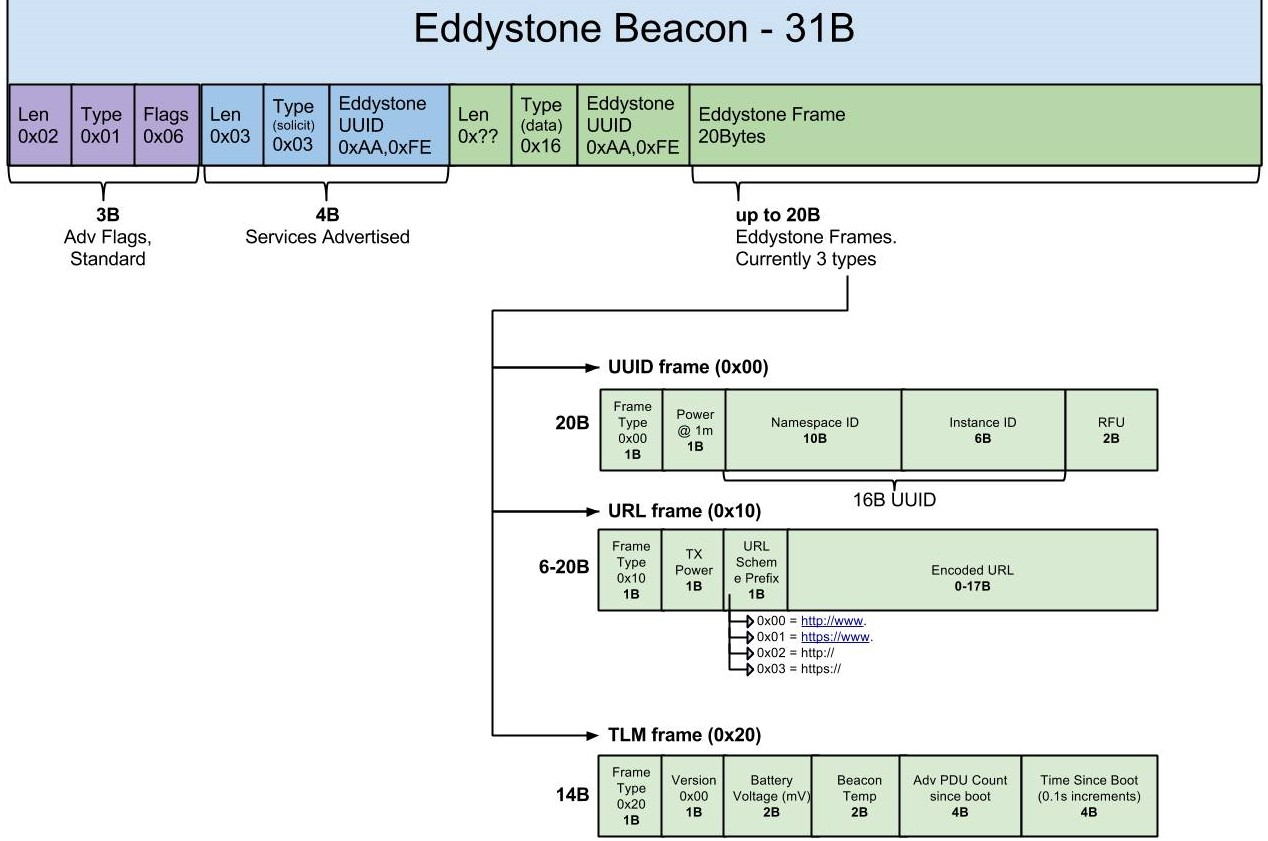
\includegraphics[scale = 0.492]{eddystone}
	\caption{This diagram shows the different Eddystone protocols and the advertising data.}
	\label{fig:eddystone}
\end{figure}
\vspace*{0cm}

\subsection{iBeacon}
The Ibeacon protocol has been the first to be released, in December 2013, by Apple. It is proprietary to the company, but it can be programmed, discovered and used also by Android applications. As the first protocol to be released, it is now the most widely supported and it is implemented in retail stores, shopping centres, airports etc... As all the other beacons it can work with any device which support Android 4.3 (Jelly Bean) or above.\\
Regarding the advertising format, it is made up of 31B Data, divided into 5 smaller values: Ibeacon Prefix, which is set by the manufacturer and cannot be modified; the UUID (Universally Unique Identifier) which can be changed and tends to represent the company's name or a particular fleet of beacons, for example, if a shopping centre buys a certain number of beacons for that specific mall, they will have the same UUID, it is was differentiate them from other beacons outside the shopping centre control. The third value will be the Major number (also adjustable), which, in the shopping mall example will represent the floor they are placed on. The fourth element is the Minor number, which identifies only one specific beacon, for example the beacon next to the coffee machine.
Lastly, but not less important, is the TxPower, which represents the Signal Strength at 1 meter from the device.
All these terms and values are shown in Figure~\ref{fig:ibeacon}

\clearpage
\begin{figure}[t!]
	\centering
	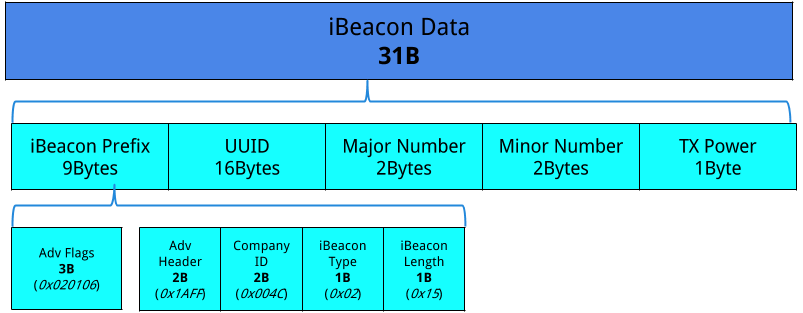
\includegraphics[scale = 1.641]{ibeacon}
	\caption{Ibeacon Advertising Protocol.}
	\label{fig:ibeacon}
\end{figure}
\vspace*{0cm}

\clearpage
\section{Indoor Trilateration}
Indoor trilateration is the method used to determine somebody's position indoors, inside a building, without the need for a GPS signal.\\
It is achieved by a variety of means. The one described here will only involve the use of beacons.\\
First of all, it would be appropriate and beneficial to briefly explain the difference between Trilateration and Triangulation, because those words might be used loosely and might be misunderstood.\\
Triangulation is a method to calculate a position using 3 or more fixed points by measuring angles, while Trilateration is based upon measuring distances. With that said, we can explore in more details how the ladder is practically achieved.\\
Let's take as an example the Figure 3.6.\\

		\begin{wrapfigure}{l}{0.4\textwidth}
		\centering
		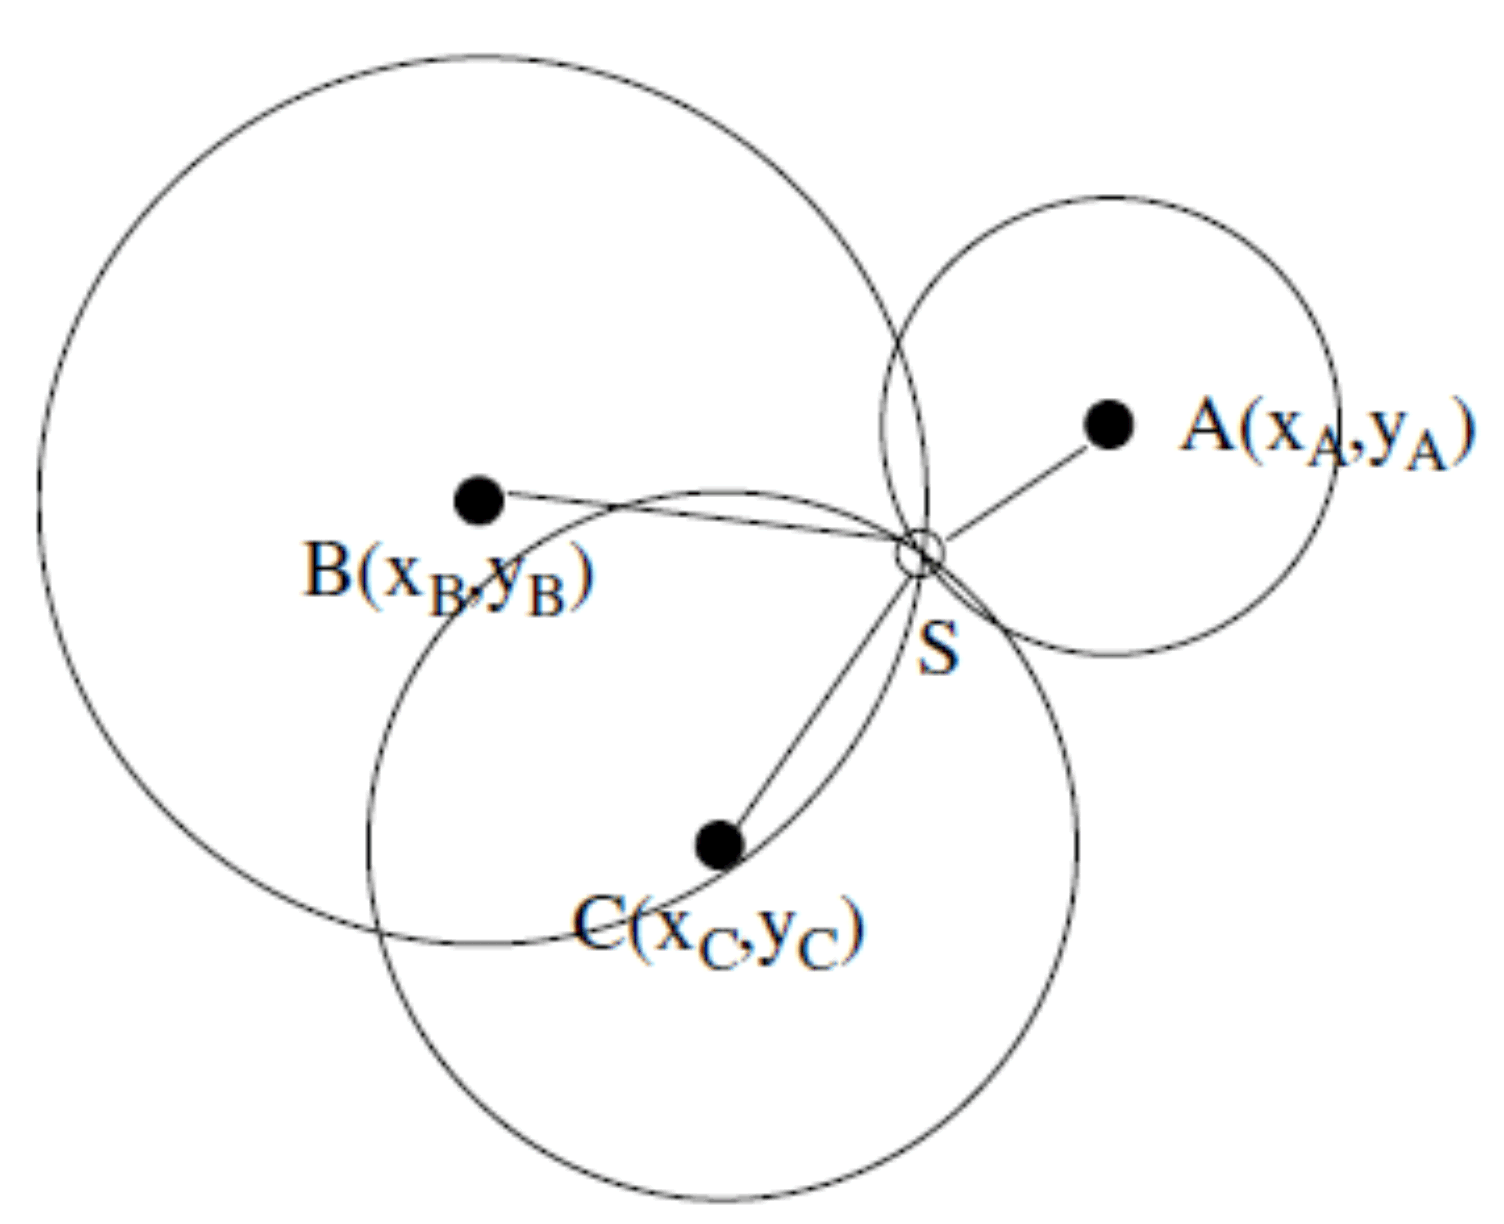
\includegraphics[width=.90\linewidth]{trilateration}
		\caption{Trilateration method shown. A,B,C represent the beacons. The circles represent the distance measured to the device.}
		\label{trilateration}
	\end{wrapfigure}

Firstly, 3 fixed points are needed; in the project scenario, 3 beacons.\\
The letter S represents the user's device, which could be a mobile phone.\\
The process starts with the receiver (S) calculating how far it stands from the beacon A; it then draws a circle whose radius is the distance measured. This means that the device is located somewhere on that circle. The issue is that the phone could be anywhere on that circle. To narrow it down, the receiver also measures the distance from the second beacon, letter B and draws the second circle consequently. Therefore now there are 2 circles, which intersect in two points. Those 2 intersections represent 2 possible positions for the mobile device. This solution is still too broad to be considered accurate and be taken into account, therefore the receiver measures the distance from the last device, C, draws the last circle, and its intersection with the other 2 represent the receiver's position.\\ 
This is how Trilateration works.\\
But how does the device actually measure distance?\\
The device must use a specific formula in order to obtain the distance from a beacon and this is the following: 
\begin{equation}
d = 10^(TxPower - RSSI)/10*n
\end{equation}
- d = distance.\\
- TxPower = actual power at which the signal is sent.\\
- RSSI = signal strength measured by the receiver.\\
- n = variable varying from 2 to 4, for most beacons is 2-2.5. Vary it depending on the situation to get a better reading.\\
\\
The formula can be slightly tweaked depending on the situation, the environment, the beacon's used, their signal strength, interference etc...\\
There are also other scenarios which must be taken into account; for example when there are only two fixed points available, therefore only two beacons. if only 2 fixed points are present, the trilateration principle of the three circles does not fully comply. Therefore, what could be done to face that problem?\\
\\

1. Fixed points in range: \\
The best solution is to take the two circles, derived from the measured distance, draw a straight line which connects the two points where these two circles intersect and find the centre of this line. The middle point will be the estimate of the receiver's location.\\\\

2. Fixed point not in range: \\
To tackle the problem the first step is to draw a straight line starting at the centre of one circle and ending at the centre of the second one. The second step is to find the middle point of the fragment of the line, which is outside of both circles. That would be the closest estimate of the distance.\\\\
(to be continued)





	






